\usetikzlibrary{patterns}

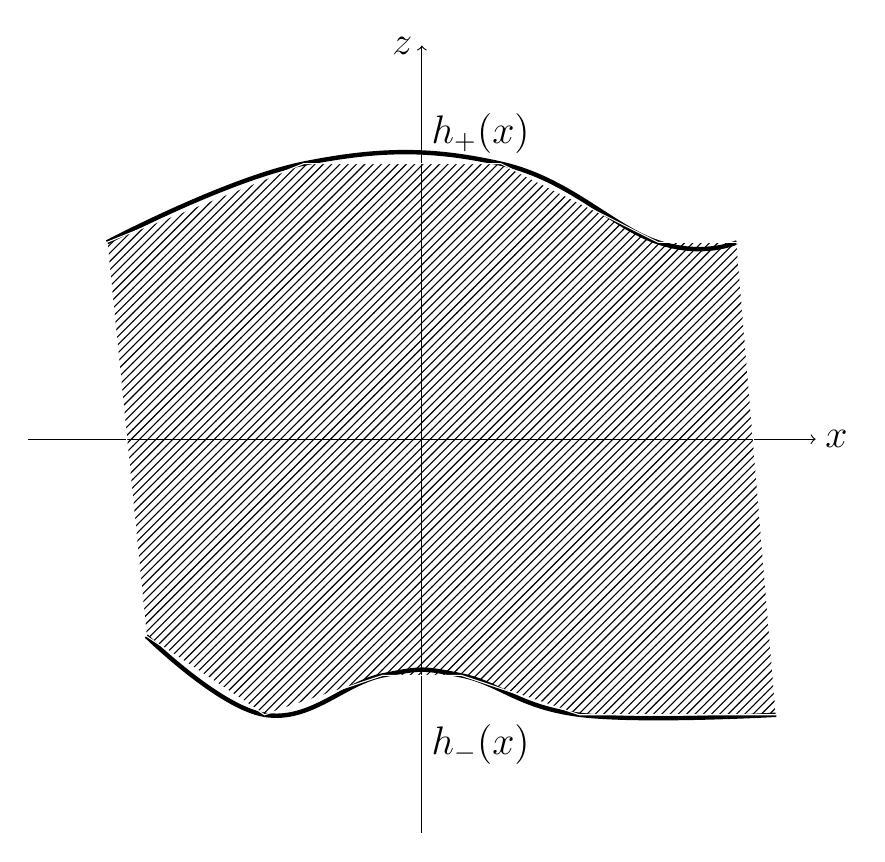
\begin{tikzpicture}

\node[coordinate] (v0) at (0,0) {};
\node[coordinate] (v1) at (-5,0) {};
\node[coordinate] (v2) at (5,0) {};
\node[coordinate] (v3) at (0,-5) {};
\node[coordinate] (v4) at (0,5) {};

\draw [->] (v1)--(v2);
\draw [->] (v3)--(v4);

\node (v5) at (-4,2.5) {};
\node (v6) at (-1.5,3.5) {};
\node (v7) at (1,3.5) {};
\node (v8) at (3,2.5) {};
\node (v9) at (4,2.5) {};
\node (v10) at (-3.5,-2.5) {};
\node (v11) at (-2,-3.5) {};
\node (v12) at (-0.5,-3) {};
\node (v13) at (0.5,-3) {};
\node (v14) at (2,-3.5) {};
\node (v15) at (4.5,-3.5) {};

\draw[ultra thick]  plot[smooth, tension=.7] coordinates {(v5) (v6) (v7) (v8) (v9)};
\draw[ultra thick]  plot[smooth, tension=.7] coordinates {(v10) (v11) (v12) (v13) (v14) (v15)};

\draw [white, pattern=north east lines, xshift=0.5cm,yshift=4.5cm] plot coordinates {(v5) (v6) (v7) (v8) (v9) (v15) (v14) (v13) (v12) (v11) (v10) (v5)};

\node [above right] at (0,3.5) {\Large \bfseries $h_{+}(x)$};
\node [below right] at (0,-3.5) {\Large \bfseries $h_{-}(x)$};
\node [right] at (5,0) {\Large \bfseries $x$};
\node [left] at (0,5) {\Large \bfseries $z$};

\end{tikzpicture}